\documentclass[output=paper]{langscibook}
\ChapterDOI{10.5281/zenodo.22796673}
\author{Ali Saeedi\orcid{https://orcid.org/0009-0007-6691-6248}\affiliation{University of Illinois Urbana-Champaign}   and Longhui Zou\orcid{https://orcid.org/0000-0002-0175-4029}\affiliation{University of Illinois Urbana-Champaign}   and Michael Carl\orcid{https://orcid.org/0000-0002-2815-0292}\affiliation{Kent State University}}
  
\title[Navigating translation effort]{Navigating translation effort through translation process research database to unravel dimensions of script and text direction}
\abstract{This chapter delves into the multifaceted interplay between different script and text direction in translation, exploring the nuanced technical, temporal, and cognitive effort exerted by translators. We utilize a methodological approach that combines eye-tracking and keylogging data with 2-way ANOVA, using a series of empirical features (such as insertion, deletion, pause-to-word ratio, total number of fixations, etc.) to measure indicators of effort in translation. The study reveals elevated effort when translating between languages with different scripts and text directions. The findings underscore that script differences may introduce challenges at orthographic, lexical, and segment levels, while text direction differences augment spatial orientation demands. Notably, while both factors individually increased translation effort, an interaction effect between script difference and text direction difference was not observed, suggesting distinct cognitive processes for each challenge. These revelations hold profound implications for translation pedagogy, advocating for tailored training approaches and the integration of specific translation strategies to navigate these difficulties. The chapter contributes empirical insights to translation research, emphasizing the pivotal role of scriptural and spatial attributes in the translation process.
\keywords{script differences, text direction, technical effort, temporal effort, cognitive effort, orthographic decoding, spatial orientation, translation pedagogy}
}
\IfFileExists{../localcommands.tex}{
  \addbibresource{../localbibliography.bib}
  \usepackage{tabularx,multicol}
\usepackage{url}
\urlstyle{same}

 
\usepackage{langsci-optional}
\usepackage{langsci-lgr}
\usepackage{langsci-gb4e}

\usepackage{paralist}
\usepackage{enumitem}
\usepackage{cprotect}
\usepackage{fancyvrb}

\let\clipbox\relax
\usepackage[export]{adjustbox}
\usepackage{array}
\usepackage[normalem]{ulem}
\usepackage{langsci-branding}
\usepackage{langsci-bidi}
\usepackage[linguistics]{forest}

  
\makeatletter
\let\thetitle\@title
\let\theauthor\@author
\makeatother

\newcommand{\togglepaper}[1][0]{
   \bibliography{../localbibliography}
   \papernote{\scriptsize\normalfont
     \theauthor.
     \titleTemp.
     To appear in:
     E. Di Tor \& Herr Rausgeberin (ed.).
     Booktitle in localcommands.tex.
     Berlin: Language Science Press. [preliminary page numbering]
   }
   \pagenumbering{roman}
   \setcounter{chapter}{#1}
   \addtocounter{chapter}{-1}
}

\newbool{bookcompile}
\booltrue{bookcompile}
\newcommand{\bookorchapter}[2]{\ifbool{bookcompile}{#1}{#2}}

\newcommand{\qual}[1]{`#1'}
\newcommand{\bv}[1]{(\ref{#1})}

\newcommand{\ip}{ImPost}
\newcommand{\ipadv}{ImPost-adverbial}
\newcommand{\pradv}{ProxPost-adverbial}
\newcommand{\chisq}{Chi-squared}


% for rotated columns
\newcolumntype{T}[2]{%
    >{\adjustbox{angle=#1,lap=\width-(#2)}\bgroup}%
    l%
    <{\egroup}%
}
\newcommand*\rot{\multicolumn{1}{T{45}{1em}}}%


\VerbatimFootnotes


% \newcommand{\keywords}[1]{\textbf{#1}}


%  \newcommand{\textarabic}[1]{\RL{\arabicfont #1}}

  %% hyphenation points for line breaks
%% Normally, automatic hyphenation in LaTeX is very good
%% If a word is mis-hyphenated, add it to this file
%%
%% add information to TeX file before \begin{document} with:
%% %% hyphenation points for line breaks
%% Normally, automatic hyphenation in LaTeX is very good
%% If a word is mis-hyphenated, add it to this file
%%
%% add information to TeX file before \begin{document} with:
%% %% hyphenation points for line breaks
%% Normally, automatic hyphenation in LaTeX is very good
%% If a word is mis-hyphenated, add it to this file
%%
%% add information to TeX file before \begin{document} with:
%% \include{localhyphenation}
\hyphenation{
    par-a-digm
}

\hyphenation{
    par-a-digm
}

\hyphenation{
    par-a-digm
}

  \togglepaper[1]%%chapternumber
}{}

% \usepackage{academicons}
% \renewcommand{\orcid}[1]{\,{\scriptsize(#1)}}
%\renewcommand{\orcid}[1]{\,{\scriptsize(\href{https://orcid.org/#1}{ORCID: #1})}}
\begin{document}
\maketitle
%\shorttitlerunninghead{}%%use this for an abridged title in the page headers



\section{Introduction}


\subsection{Research background}

The process of translation is influenced by a myriad of factors (\citealt{Marmaridou1996}; \citealt{Campbell1999}; \citealt{Sun2015}; \citealt{Screen2016};  \citealt{RojoLópezEtAl2021}; \citealt{ZouEtAl2022}), among which script and text direction of the language pairs involved play a role (\citealt{saeedi_cognitive_2022}). Nevertheless, most research that relates script and text direction to the cognitive process mainly revolves around topics of bilingualism, second language learning, reading comprehension, and information processing, among others, but not translation studies (\citealt{Aro2004}; \citealt{BarrettEtAl2002}; \citealt{Boroditsky2001}; \citealt{ChatterjeeEtAl1999}; \citealt{SpalekHammad2005}). For instance, in bilingualism research, \citet{DuñabeitiaEtAl2009} reported increased priming effects when dealing with words of similar orthographical representations in two languages of the similar script compared to dealing with words of dissimilar orthographical representations in these two languages (e.g., Arabic (en)-> Arabica (es); Dutch (en)-> Holandesa (es)). Other findings from many studies in the fields of reading and information processing have shown effects of native language orientation and text direction on spatial bias in reading comprehension. For instance, readers accustomed to left-to-right-oriented scripts, such as English, and those familiar with right-to-left-oriented scripts, like Arabic, exhibit biases that correspond to their respective text directions \citep{Mashat2017}.

As for translation process research, much research has focused on the relationship between different aspects of language specificity (i.e., unique characteristics, nuances, and idiosyncrasies of a particular language pair that can influence the translation process) (see \citealt{Campbell1999}; \citealt{Gile2005}, \citealt{gile_2008}; \citealt{WangZou2018}; \citealt{ZouEtAl2022}) and translation difficulty but not on the language script and text direction. Some of these studies linked specific linguistic features like lexical and syntactic complexity to translation difficulty (e.g., \citealt{VanroyEtAl2021}; \citealt{ZouEtAl2021}). However, little work has focused on how differences in writing systems and text orientations influence the translation process. Whenever mentioned, studies state that language pairs with different scripts or text directions are expected to entail greater efforts, compared to languages with similar script and same text direction. \citet{LacruzEtAl2016} for instance, posited that language pairs with differing scripts involve increased cognitive effort during the translation process compared to language pairs with similar scripts. The underlying rationale might be that the visual-spatial differences in scripts can introduce additional layers of complexity, requiring translators to navigate the apparent differences in the orthographic features of each script. Hence, there remains a conspicuous gap, specifically, on the interplay between script, text direction, and translation difficulty. This gap is even more pronounced when juxtaposing different language pairs, such as translations from English into Spanish, English into Chinese, and English into Arabic, in the context of their script and directional attributes. Building on this gap, the nuanced interrelations between script, text direction, and exerted effort in translation warrant deeper exploration.

\subsection{Research purpose}

This study aims to examine how different scripts and text direction between language pairs impact the effort involved in translation. This would reveal the inherent complexities faced by translators when bridging languages that employ diverse symbolic representations and reading and writing directions. Specifically, we compare the translation process from English into three different target languages: Spanish, Simplified Chinese, and Arabic. Spanish shares the same Modern Latin alphabet with English and has left-to-right text direction. Simplified Chinese utilizes logographic characters and left-to-right text direction. Arabic has a cursive Abjad script written right-to-left. By comparing the translation process of different language pairs, we can determine if variations in script and text direction increase effort.

Script disparities require utilizing distinct visual-spatial pathways and cognitive resources (\citealt{KandhadaiFedermeier2010}; \citealt{PerfettiEtAl2007}). This likely increases the cognitive load for translators, but there is a lack of research directly testing this hypothesis. Beyond scripts, flipping text direction may involve extra spatial processing and attention shifting, such as left-to-right (e.g., English) versus right-to-left (e.g., Arabic). Contrasting our three language pairs allows investigation of these two variables. Spanish acts as a control, while Chinese exemplifies different script but same text direction as English and Arabic both different script and different text direction.

Demonstrating increased difficulty for the Chinese and Arabic pairs would have important theoretical and practical implications. It would empirically validate the influence of script and text direction on the cognitive translation process. Theoretically, this helps advance models of how language systems interact during translation. Practically, it suggests value in developing specialized pedagogical approaches tailored to teaching translation between dissimilar scripts and text directions. For Chinese, this may involve an added focus on strategies for converting between logographic and alphabetic systems during the translation process, like engaging in holistic visual-spatial processing of extended chunks of Chinese logograms during translation and mapping meaning across writing systems. For Arabic, emphasis could be placed on mastering the intricacies of its right-to-left script progression, coupled with exercises that delve into the nuances of its phonetic, morphological and syntactic structures, and activities designed to enhance spatial attention adaptation to its unique cursive and diacritical features.

Our study utilizes eye-tracking and keylogging data of from-scratch translation experiments. We hypothesize English-into-Spanish translation would show relatively less effort due to shared script and text direction. English into Chinese and English into Arabic are expected to show an increased effort due to different scripts and, in case of Arabic, additionally, reversed text direction. By pinpointing the challenges and proposing tailored strategies, our study represents an essential step toward better understanding and facilitating the quality and efficiency of translations across genetically distant languages \citep{Xiao2010}. Consequently, this chapter attempts to address the following research questions:

\ea
Does translating from a source text (ST) to a target text (TT) of different scripts (e.g., English into Chinese/Arabic) require more translation effort than translating between languages with similar scripts (e.g., English into Spanish)? 
\z
\ea
Does the difference in text direction between the languages (e.g., English into Arabic) contribute to an increased effort in translation? 
\z
\ea
Is there an interaction effect between the script difference and text direction difference on the cognitive effort during the translation process?
\z

\subsection{{Methodology}  }

\subsection{Datasets description}

This study utilizes eye-tracking and keylogging data from three existing datasets available at the Center for Research and Innovation in Translation and Translation Technology’s Translation Process Research Database (CRITT TPR-DB) \citep{CarlEtAl2016}.\footnote{The CRITT TPR-DB consists of studies that were conducted with Translog-II, Trados or with the CASMACAT workbench. Behavioral and textual data from translation experiments is publicly available, and a list of publications utilizing this database is accessible on the CRITT@kent website: https://sites.google.com/site/centretranslationinnovation/tpr-db/public-studies} The datasets are BML12 (English into Spanish), RUC17 (English into Simplified Chinese), and AR19 (English into Arabic). The three datasets contain sessions of different tasks (from-scratch translation, post-editing, sight translation, etc.). We only use the from-scratch translation sessions for the purpose of this study. These three datasets involve an identical set of English STs, thus the linguistic complexity of the STs is identical among all datasets. The STs include six English texts from Encyclopedia (four news articles and two sociology articles). The STs comprise a total of 847 words over 41 segments on the sentence level. A detailed breakdown of segments and words for each ST is outlined in \tabref{tab:saedi:1}.

\begin{table}
\begin{tabularx}{\textwidth}{Xrrrrrrr}
\lsptoprule
  {Source text} & {1} & {2} & {3} & {4} & {5} & {6} & {Total}\\
  \midrule
  {Source segments} & 11 & 7 & 5 & 5 & 6 & 7 & 41~\\
  {Source words} & 160 & 153 & 146 & 110 & 139 & 139 & 847~\\
\lspbottomrule
\end{tabularx}
\caption{\label{tab:saedi:1}Breakdown of segments and words for the six source texts.}
\end{table}

English-into-Spanish dataset (BML12): This dataset encompasses 32 translators, all of whom are native Spanish speakers. It serves as the baseline condition, since Spanish shares the same Latin alphabet and left-to-right direction as English. The gaze data was collected using a Tobii T60 remote eye-tracker.

English-into-Simplified Chinese dataset (RUC17): This dataset contains data from 21 translators, all native Chinese speakers. It represents a language pair with different scripts but the same text direction since simplified Chinese uses logographic script and generally maintains left-to-right text direction. The gaze data was recorded using a Tobii TX300 eye-tracker.

English-into-Arabic dataset (AR19): This dataset includes 22 translators, all of whom are native Arabic speakers. The gaze data was collected with an SMI iView eye-tracker.

The keystroke logging data was collected using Translog-II for all datasets. All translators in these three datasets have English as their second language and are native speakers of their respective target language. In total, there are 162 translation sessions consisting of 1,116 individual segments in this research. As can be seen in \tabref{tab:saedi:2}, the number of sessions and segments of English-into-Spanish (BML12) and English-into-Chinese (RUC12) datasets are in closer range compared to a smaller number for the English-into-Arabic dataset (AR19). Therefore, we normalize the data by the number of ST words on the segment level for comparable analysis. An interesting observation here is that, proportionally speaking, the number of target words and characters for the English-into-Spanish dataset (BML12) is remarkably higher than both the English-into-Chinese dataset (RUC17) and the English-into-Arabic dataset (AR19). We delve into a discussion about the correlation of such divergence with technical and temporal effort in section \ref{bkm:Ref148304982} (Results and Discussion) of this chapter (see subsections \ref{bkm:Ref148304918}., \ref{bkm:Ref148304935}., \ref{bkm:Ref148304950}., and \ref{bkm:Ref148304962}.).

\begin{table}
\begin{tabularx}{\textwidth}{p{1.3cm}YYYY}
\lsptoprule
 {Datasets} & {Number of sessions} & {Number of segments} & {Number of target words} & {Number of target characters}\\
 \midrule
{ {BML12}}

 {(en-es)} & 60 & 411 & 10,050 & 56,936~\\
{ {RUC17}}

 {(en-zh)} & 62 & 428 & 8,507 & 14,470~\\
{ {AR19}}

 {(en-ar)} & 40 & 277 & 6,131 & 33,276~\\
 {Total} & 162 & 1,116 & 24,688 & 104,682~\\
\lspbottomrule
\end{tabularx}
\caption{\label{tab:saedi:2}Detailed description of the three datasets.}
\end{table}

\subsection{Grouping language pairs for analysis}

One of the primary aims of this chapter is to dissect the influence of script and text direction on translation effort. To this end, we initially compare the translation process of English-into-Spanish against the other two language pairs (English-into-Chinese and English-into-Arabic) to isolate and examine the impact of script differences. This comparison is pivotal as English and Spanish have similar scripts and the same text direction, offering a baseline for assessing the additional effort introduced by different scripts. Subsequently, we combine English-into-Spanish and English-into-Chinese into a group to focus on the impact of text direction differences in comparison to English-into-Arabic. This methodological decision stems from the need to separately evaluate the influence of the two independent variables, script, and text direction, where English-into-Arabic is distinct in both aspects. By comparing this combined group against English-into-Arabic, we aim to isolate and scrutinize the translation effort attributed solely to the opposite text direction. This strategic grouping allows for a nuanced analysis of how each factor—script and text direction—contributes to the overall translation effort, while also considering their interaction effect.

\subsection{Indicators of translation effort}

Several indicators have been meticulously examined to gauge the intricacies of translation effort at the segment level in this chapter. These indicators are selected according to Krings’ categorization of technical, temporal, and cognitive efforts \citep{krings_repairing_2001}. While this framework was developed to better understand and measure the challenges faced by translators, especially in the context of post-editing machine translation outputs, they collectively provide a holistic view of the multifaceted effort involved in the translation process \citep{CarlEtAl2022}. Therefore, this framework is utilized herein for from-scratch translation data. These effort indicators are measured relying on several features available in the CRITT TPR-DB \citep{CarlEtAl2016}. Technical effort primarily focuses on the tangible modifications made during the translation process. This includes the insertion keystrokes (“Ins”), the deletion of existing characters (“Del”), and the overall number of revisions made to the segment (“Nedits”). These metrics provide a straightforward measure of the manual adjustments a translator makes at the segment level. Temporal effort is encapsulated by the “DurLog” metric, which is calculated by the logarithm of the duration spent on translating the segment.

The cognitive effort involved in translation is perhaps the most intricate to measure, given its intangible nature. One of the primary metrics we use in this chapter is pause-to-word ratio (“PWR”), which stands for the number of pauses per word in a segment. PWR is a measure of cognitive effort mainly developed in machine translation post-editing, although it has been applied to assess cognitive effort in from-scratch translation (\citealt{LacruzEtAl2016}; \citealt{LacruzEtAl2018}).  Another set of metrics that offer insights into cognitive effort are “FixS” and “FixT”, which represent the total number of fixations on the STs and TTs. These fixation counts offer a quantitative measure of the attention and focus a translator directs towards the STs and TTs during the translation process. Complementing the fixation metrics are “TrtS” and “TrtT”, which stand for the total reading time on the STs and TTs, respectively. These metrics capture the total of all fixation durations on the ST side or the TT side of certain segment, irrespective of when these occurred during the session. In essence, they provide a measure of the time a translator spends comprehending and processing both the STs and TTs.

Lastly, the concept of translation entropy is introduced through the “HTot” metric. HTot, at the segment level, denotes the total translation entropy of a source segment \citep{Carl2021}. HTot measures segment-level entropy by integrating HTra (word translation entropy) and HCross (entropy of the Cross value). It assesses the variation concerning both word choice and word ordering (\citealt{CarlSchaeffer2017}). For the indicators of cognitive effort in translation, two-way ANOVAs are conducted with script (similar vs. different) and text direction (same vs. opposite) serving as independent variables. This allows analysis of the main effects of script and text direction and their interaction effect on translation effort. To this end, the dependent variable HTot is chosen as the primary measure for our analysis due to its comprehensive nature, reflecting both word translation entropy and the entropy of Cross value. This measure’s ability to integrate various aspects of cognitive effort renders it particularly suitable for examining translation difficulty. In addition to HTot, we consider PWR, FixS, FixT, TrtS, and TrtT. The selection of HTot does not preclude the relevance of these indicators; rather, it underscores our methodological decision to anchor our analysis in a variable that encapsulates the multifaceted nature of translation effort.

\subsection{{Results}  {and}  {discussion}}

\label{bkm:Ref148304982}

In our analysis, we used the Mann-Whitney U test to assess the statistical significance of the differences observed between groups across our measures of effort. In this chapter, we focus on discussing results from measures that demonstrated significant differences, as they are of relevance to our research questions and contribute meaningful insights into the impact of script and text direction on translation effort. Non-significant results, while part of the comprehensive analysis, are not elaborated upon here, as they do not substantively alter the interpretation of our primary findings.

\subsection{Script}

\label{bkm:Ref148304918}
\subsubsection{{Script} {and} {technical} {effort}}

In examining the technical effort associated with script, we analyzed metrics of insertion (Ins), deletion (Del), and the number of revisions (Nedit) per ST token as \figref{fig:saedi:1} shows. For the English-into-Spanish dataset with similar script, these metrics are represented in the blue plot boxes (SScript), while the English-into-Chinese and English-into-Arabic datasets with different scripts are depicted in the orange plot boxes (NScript). Notably, the data indicates that the language pair with similar scripts exhibits a higher frequency of insertions, deletions, and number of revisions compared to the insertions, deletions, and number of revisions of language pairs with different scripts. This observation aligns with the disparities in target word and character counts among the datasets, as shown in \tabref{tab:saedi:2}. Such findings underscore an increased technical effort inherent to the similar-script dataset relative to its different-script counterparts.

\begin{figure}
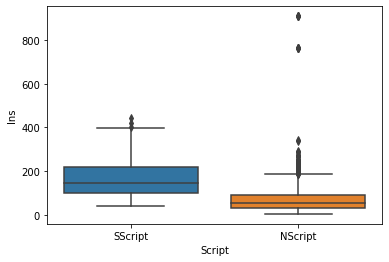
\includegraphics[height=.3\textheight]{figures/a2Saedietal-img001.png}
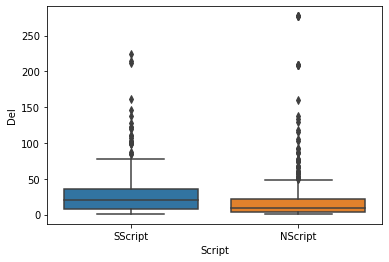
\includegraphics[height=.3\textheight]{figures/a2Saedietal-img002.png}
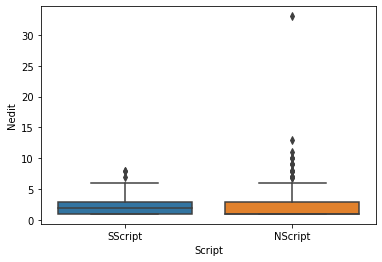
\includegraphics[height=.3\textheight]{figures/a2Saedietal-img003.png}
\caption{\label{fig:saedi:1}\label{bkm:Ref148304841} Insertion, deletion, and number of revisions for similar-script and different-script language pairs.}
\end{figure}

At first glance, one might assume that translations between languages with similar script would be more straightforward, given the shared orthographic features. Yet, our results challenge this assumption, showing higher technical effort in terms of insertions, deletions, and revisions for the similar-script English-into-Spanish dataset compared to the different-script datasets. In addition to the variations in word length among languages, a possible reason is that the higher degree of lexical similarity found between languages that are closely related (such as English and Spanish) introduces more opportunities for ambiguity that needs to be resolved in the translation process. Many words in both languages have similar orthography and phonetics. This can lead to negative priming effect manifested in a myriad of phenomena such as “false friends” – words that look or sound similar in both languages but have different meanings. Such similarities can lead to confusion and require careful handling during translation (\citealt{GrangerSwallow1988}). In our English-into-Spanish dataset (BML12), the English source word ‘increases’ for instance was translated by half of the translators into Spanish using an iteration of the target word ‘\textit{incrementos’} and later edited into an iteration of the target word ‘\textit{aumen}’. This introduced an average of 12.25 insertions, 3.13 deletions, and 15.38 edits per English-into-Spanish translator for the translation of this source word in our dataset.

In contrast, when translating between languages with different scripts (e.g., English-into-Chinese and English-into-Arabic), there is less likelihood of confusion due to “false friends” or orthographically or phonetically similar words. The challenges here lie more in understanding the structure, context, and nuances of the source and target languages. The English-into-Arabic dataset (AR19) shows that the source word ‘increases’ was translated by all the translators into an iteration of the target word ‘{\arabicfont زيادة}’\normalfont (‘increase’). The average number of insertions was 6.9, 1.42 for deletions, and 8.32 for edits per English-into-Arabic translator for this word, which are significantly lower averages than English-into-Spanish. By the same token, English-into-Chinese translators translated the source word ‘increases’ into an iteration of the target word ‘{\cn 上涨}’ (‘rise’) with minimal edits. The average number of insertions per translator was 2.75, 0 for deletions, and 2.75 for edits for this word. Additionally, the divergence in target word and character counts, as mentioned, might also reflect the inherent challenges of linguistic transfer between similar-script languages. This echoes findings from previous studies like (\citealt{RojoLópezEtAl2021}), which suggest that higher familiarity can sometimes lead to increased challenges in translation.

\subsubsection{{Script} {and} {temporal} {effort}          }
\label{bkm:Ref148304935}

As for the analysis of temporal effort in regard to script, we took the DurLog metric as the indicator of effort. In \figref{fig:saedi:2}, the red line in the histogram refers to the logarithm of production duration for the similar-script English-into-Spanish dataset (Sscript), while the blue line refers to the different-script English-into-Chinese and English-into-Arabic datasets (Nscript). We can see that translation with the similar-script language pair generally takes less time and eventually less temporal effort than the different-script language pairs. This is an interesting finding given the fact that English-into-Spanish sessions tend to have more insertions, deletions, and number of revisions; still they are faster.

\begin{figure}
\label{bkm:Ref148305240}
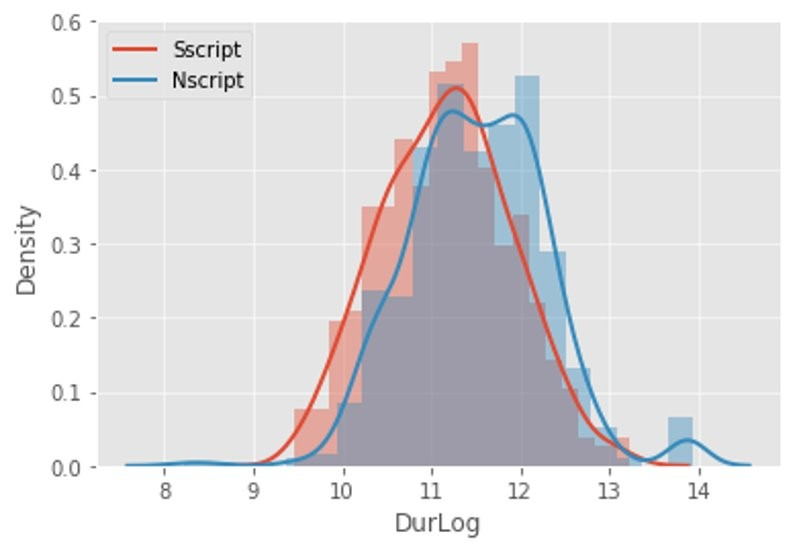
\includegraphics[height=.3\textheight]{figures/a2Saedietal-img004.jpg}
\caption{\label{fig:saedi:2} Production duration for similar-scripts and different-scripts language pairs.}
\end{figure}

The temporal effort analysis adds another layer to our understanding of the nuances involved in translation across different scripts. While the similar-script English-into-Spanish dataset exhibits higher technical effort in terms of insertions, deletions, and overall revisions, it intriguingly requires less temporal effort. This finding might be reminiscent of the “familiarity and fluency” observed in cognitive psychology, where familiarity with a task can lead to quicker completion, even if the task involves more steps or corrections (\citealt{AlterOppenheimer2008}). In the context of translation, translators working with similar scripts might experience an increased fluency in reading and processing the ST, allowing them to translate faster despite the increased technical effort. Moreover, these findings might suggest different cognitive load on translators \citep{Sweller2011}. The different scripts of Chinese and Arabic could introduce an additional layer of cognitive load on the translators, slowing down their translation speed. On the other hand, while Spanish and English have similar scripts, the translators might be leveraging their familiarity to process information quickly, even if it entails more edits. This dynamic interplay between technical and temporal efforts underscores the multifaceted nature of translation processes and highlights the importance of considering multiple dimensions of effort when analyzing translation tasks.

\subsection{{Script} {and} {cognitive} {effort}}

Focusing on the cognitive effort, we take several indicators for our analysis. The first of which is pause-to-word ratio (PWR). As seen in \figref{fig:saedi:3}, the blue plot box of the similar-script English-into-Spanish (SScript) pause-to-word ratio (PWR) is lower than that of the orange plot box of the different-script English-into-Chinese and English-into-Arabic (NScript). To determine the statistical significance of the differences in PWR, we conducted the Mann-Whitney U test. The results revealed a significant difference (p < 0.05) between the SScript and NScript groups, suggesting that script differences indeed contribute to the cognitive effort in translation tasks. This would be an indicator of more cognitive effort exerted by the different-script language-pair translators compared to the similar-script language-pair translators.

\begin{figure}
\label{bkm:Ref148305336}  
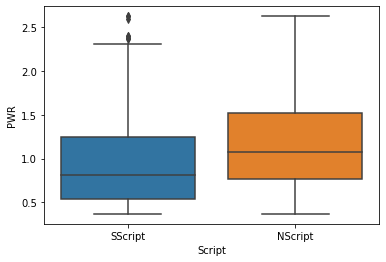
\includegraphics[height=.3\textheight]{figures/a2Saedietal-img005.png}
\caption{\label{fig:saedi:3} Pause-to-word ratio for similar-script and different-script language pairs}
\end{figure}

Pause durations in translation have been frequently associated with cognitive effort, with longer pauses typically reflecting increased cognitive effort or decision-making processes \citep{Dragsted2005}. The elevated PWR observed for the different-script language pairs (English-into-Chinese and English-into-Arabic) can be seen as a manifestation of the added cognitive challenges that these translators encounter, potentially due to the script differences. The lower PWR for the similar-script English-into-Spanish translations, despite its increased technical effort as discussed earlier, might indicate a smoother cognitive flow in terms of processing and decision-making. This smoother flow could be attributed to the orthographic familiarity between English and Spanish, which reduces the cognitive load of script decoding and allows translators to focus more on meaning transfer. Such findings underscore the nuanced ways in which script differences can modulate the cognitive load of translation, reaffirming the importance of orthographic considerations in translation research and training (\citealt{saeedi_effect_2022}).

The next cognitive effort indicators are the total number of fixations on the ST (FixS) and the total number of fixations on the TT (FixT). On the left side of \figref{fig:saedi:4}, FixS results align with PWR results and more visibly suggest less cognitive effort in general for the similar-script language pair in blue plot box (SScript) compared to the different-script language pairs in green plot box (NScript). As for FixT, as shown on the right side of \figref{fig:saedi:4}, the similar-script language pair in blue in the histogram (Sscript) show more variant effort than the different-script language pairs in orange (Nscript).

\begin{figure}
\label{bkm:Ref148305429}  
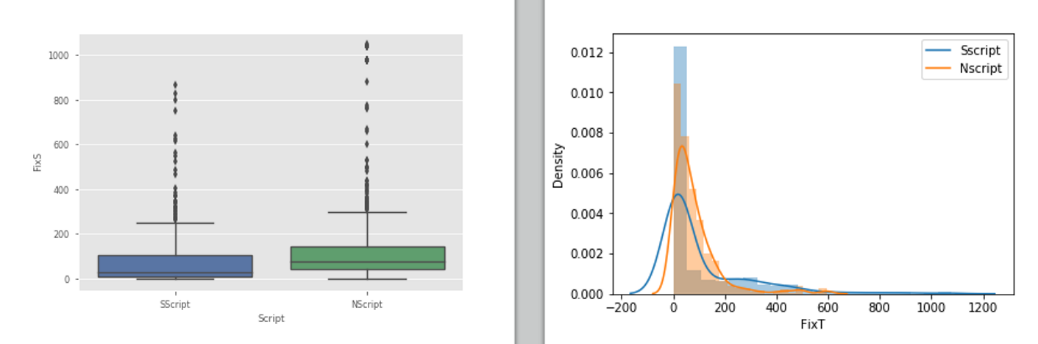
\includegraphics[width=\textwidth]{figures/a2Saedietal-img006.png}
\caption{\label{fig:saedi:4}  The total number of fixations on the source text and target text for similar-script and different-script language pairs}
\end{figure}

This suggests that the different-script language pairs require more cognitive effort, particularly evident in the increased fixations on the ST (FixS). This may indicate the nuanced challenges of processing a source language that diverges in script from the target language, especially given the fact that translators’ second language of command (L2) is English (the ST). On the other hand, the variability in fixations on the TT (FixT) for the similar-script language pair suggests that translators might be engaging in meticulous self-monitoring and revisions. Conversely, the less variation of fixations on the TT for different-script language pairs might suggest the translators’ overall familiarity with TT scripts given the TTs are their first language of command (L1). It may also underscore a consistent pattern of cognitive effort exerted in navigating between the source and target scripts during the translation process.

Another set of cognitive effort indicators is the total reading time on the ST (TrtS) showing on the left side of \figref{fig:saedi:5} and the total reading time on the TT (TrtT) showing on the right side of \figref{fig:saedi:5}. For both, we can still see lower values for the similar-script English-into-Spanish language pair as shown on the left blue plot boxes in each graph (SScript) compared to the different-script language pairs on the right side of each graph (NScript). This is yet another marker of differences in cognitive effort that might be attributed to orthographical effects.

\begin{figure}
\label{bkm:Ref148305473}  
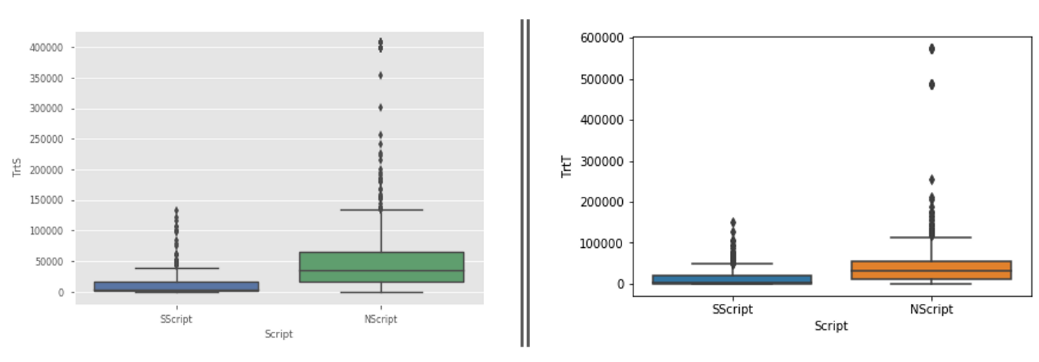
\includegraphics[width=\textwidth]{figures/a2Saedietal-img007.png}
\caption{\label{fig:saedi:5} Total reading time on the source and target for similar-scripts and different-scripts language pairs}
\end{figure}

Extended reading time has been associated with increased cognitive effort in translation (\citealt{GileLei2020}). The shorter reading time for the similar-script English-into-Spanish translations, as compared to the different-script pairs, reinforces our earlier observations of reduced cognitive effort due to script familiarity. The consistency across multiple indicators of cognitive effort -- PWR, fixations, and now reading times -- suggests that the degree of orthographic similarity significantly impacts the cognitive effort of translation, streamlining processes when scripts are aligned and adding layers of translation difficulty when they differ.

The last indicator of cognitive effort for script incorporated here is the normalized HTot. \figref{fig:saedi:6} shows a lower variation in the translation (HTotN) for the similar-script English-into-Spanish language pair in blue (SScript) compared to the different-script language pairs in orange (NScript).

\begin{figure}
\label{bkm:Ref148305555}  
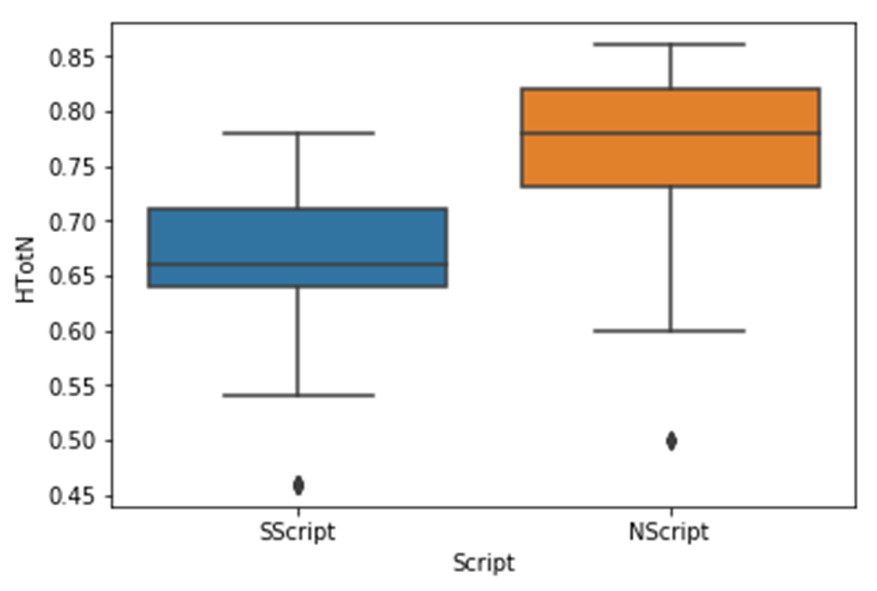
\includegraphics[height=.3\textheight]{figures/a2Saedietal-img008.png}
\caption{\label{fig:saedi:6} Normalized HTot for similar-scripts and different-scripts language pairs}
\end{figure}

The normalized HTot represents the average joint probability over alternative translations of a segment. As seen in \figref{fig:saedi:6}, the similar-script English-into-Spanish translations demonstrate less variation in HTotN, suggesting a more consistent and potentially less effortful translation process when compared to different-script pairs. Results from all these measures of cognitive effort consistently point toward the pivotal role of orthographic similarities and differences in translation difficulty. Increased variation in such probabilistic measures indicates a broader range of potential translations or more cognitive effort in selecting among alternatives \citep{SchaefferEtAl2016}. The reduced variation for the similar-script pair might indicate that overall, translators face fewer ambiguities or alternatives, potentially due to the script and linguistic similarities.

In analyzing the translations of our source English sentence “Sociology is a relatively new academic discipline” into Spanish, Chinese, and Arabic, we observe notable differences impacted by word choice rather than word order. The Spanish translation, “\textit{La sociología es una disciplina académica relativamente nueva,}” closely mirrors the English sentence in vocabulary but differs in word order, Conversely, the Chinese translation “{\cn 社会学是一门相对较新的学科}” (Shèhuìxué shì yī mén xiāngduì jiào xīn de xuékē) diverges in word choice when compared to English although order is quite similar. The Arabic translation
(
\RL{
\arabicfont
علم الاجتماع هو من العلوم الاكاديمية الحديثة نسبياً
}
\normalfont
‘Ilm al-ijtimā‘ huwa min al-‘ulūm al-akādīmīyah al-ḥadīthah nasbiyan) also introduces significant variations in lexical choice but not in word order. Juxtaposing these observations with the findings of HTotN may underscore how lexical variations influence translation effort, irrespective of the syntactic alignment between the target languages and the source language. The similarities and differences in word choice can be attributed to those in the scripts of these languages.

From our various cognitive indicators, the consistent findings of higher cognitive effort associated with differences in scripts between the language pair underscore the distinct challenges faced when translating between different scripts. These insights have direct implications for translator training. Given the pronounced cognitive effort associated with different-script language pairs, it is imperative for translation curricula to incorporate tailored modules that equip student translators with strategies to address these challenges. Educators must highlight the cognitive intricacies linked to script variations, ensuring student translators are aware of and become proficient in tackling this layer of translation difficulty both technically and cognitively. Moreover, integrating practical sessions, for instance intensive training on the proficiency of the L2 and transfer speed between the L1 and L2 on both lexical and phrasal level, can better prepare student translators for real-world translation tasks. Embracing advanced technological tools, such as specific terminology management tools, translation memories or AI-assisted translation tools, can further ease the challenges posed by script differences.

\subsection{Text direction}

\label{bkm:Ref148304950}
\subsubsection{{Text} {direction} {and} {technical} {effort}}

We repeat the same analysis procedures with text direction by comparing the datasets with language pairs sharing the same left-to-right text direction (English-into-Spanish and English-into-Chinese) to the dataset with language pair of different text directions (English-into-Arabic) since Arabic has a right-to-left writing system. For the technical effort indicators, all the indicators such as insertions (Ins), deletions (Del), and number of revisions (Nedit) generally show less variant technical effort for the same-direction datasets shown on the left side of each graph (SDirec) in \figref{fig:saedi:7} when compared to the different-direction dataset shown on the right side of each graph (NDirec).

\begin{figure}
\label{bkm:Ref148305620}  
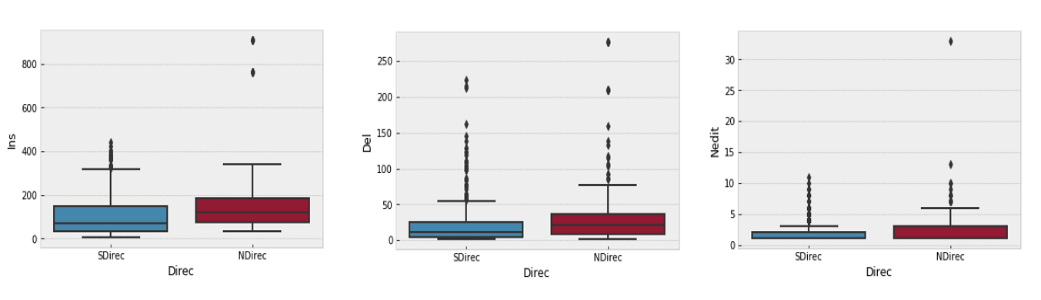
\includegraphics[width=\textwidth]{figures/a2Saedietal-img009.png}
\caption{\label{fig:saedi:7}   Insertion, deletion, and number of revisions for same-text-direction and different-text-direction language pairs}
\end{figure}

Variations in text direction, particularly between left-to-right and right-to-left writing systems, have been posited to introduce unique cognitive challenges \citep{FernandesEtAl2013}. Our findings suggest that translating between languages with the same text direction (English-into-Spanish and English-into-Chinese) leads to a less varied technical effort, in terms of insertions, deletions, and overall revisions, compared to translations involving directionally divergent scripts (English-into-Arabic). Text direction has been observed to influence various cognitive tasks, with right-to-left readers often employing different spatial and sequential processing strategies compared to left-to-right readers (\citealt{ChokronImbert1993}). The less variance in technical effort for the same-direction datasets might be attributed to the relative ease of transferring information within the same spatial framework. In contrast, translating into a language with a divergent text direction, such as Arabic, might introduce additional cognitive load, necessitating more varied technical interventions to translation production.

In addition to analyzing metrics such as insertion (Ins), deletion (Del), and number of revisions (Nedit) per ST token, we further examined the technical effort using a measure of the number of insertions divided by the number of deletions per segment. We found that language pairs with the same text direction exhibited a higher ratio of insertions to deletions per segment (10.31) compared to language pairs with different text directions (9.95). This result suggests that maintaining consistent spatial frameworks in translation, such as left-to-right or right-to-left orientation, can impact the distribution of technical effort. The lower ratio observed for language pairs with different text directions may reflect the additional cognitive load associated with transferring information across divergent spatial frameworks, highlighting the complexity inherent in translations involving directional divergence.

\section{{Text} {direction} {and} {temporal} {effort}}
\label{bkm:Ref148304962}

For the temporal effort, we see the same-direction language pairs in blue (SDirec) in \figref{fig:saedi:8} generally take less time (DurLog) than the different-direction language pair in orange (NDirec). This might suggest that Spanish and Chinese translators have less temporal effort than the Arabic translators.

\begin{figure}
\label{bkm:Ref148305751}
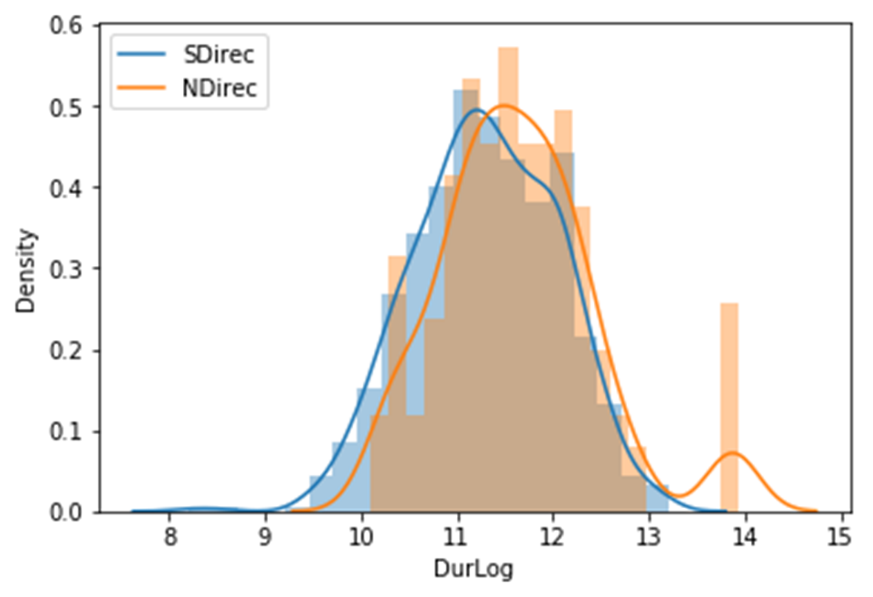
\includegraphics[height=.3\textheight]{figures/a2Saedietal-img010.png}
\caption{\label{fig:saedi:8} Production duration for same-direction and different-direction language pairs}
\end{figure}

The more condensed durations for the same-direction language pairs (English-into-Spanish and English-into-Chinese) in comparison to the different-direction English-into-Arabic pair substantiates the argument that text direction can significantly modulate the time dimensions of translation processes. Prior research has highlighted that text direction can impact reading and processing speeds \citep{Eviatar1997}. Mismatches in text direction would therefore introduce additional cognitive load, especially during the drafting and revision stages of translation. The observed temporal disparities might be attributed to the inherent challenges of adjusting from a left-to-right writing system to a reversed spatial framework in right-to-left system, such as from English into Arabic. The additional translation durations for English-into-Arabic translations may reflect the extra effort required for spatial orientation adjustments while drafting right-to-left TT. Moreover, translators may have iteratively relocated between the ST and TT during translation refinement to ensure accuracy and fluency when translating into the opposite text direction.


\section{{Text} {direction} {and} {cognitive} {effort}}

Like our analysis of script effects, the first cognitive effort measure we examine in relation to text direction is PWR. As can be seen in \figref{fig:saedi:9}, the PWR shows less variation for the same-direction language pairs in blue (SDirec) and more variation for the different-direction language pair in red (NDirec).

\begin{figure}
\label{bkm:Ref148305797}
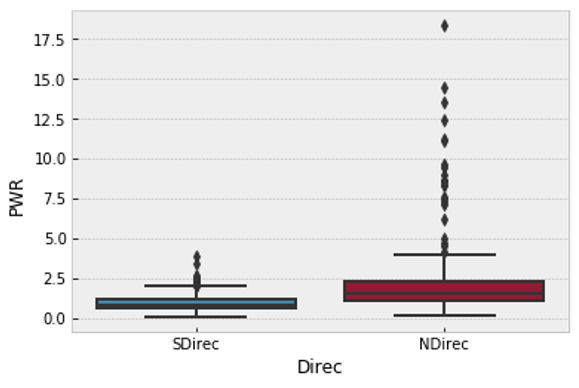
\includegraphics[height=.3\textheight]{figures/a2Saedietal-img011.png}
\caption{\label{fig:saedi:9}  Pause-to-word ratio for same-direction and different-direction language pairs}
\end{figure}

The attenuated variation in PWR for the same-direction language pairs (English-into-Spanish and English-into-Chinese) suggests a more streamlined cognitive trajectory during the translation process. In contrast, the heightened variation for the different-direction English-into-Arabic language pair may be an indicative of the additional cognitive challenges posed by directional disparities. Our findings suggest that translating between different text directions (left-to-right into right-to-left) poses asymmetric cognitive challenges for translators. They must grapple with lexical and syntactic transfers while also realigning spatially to the opposite right-to-left text direction. This appears to create fluctuations in pause duration as translators navigate these linguistic and spatial difficulties. The additional cognitive effort required to translate from a different text direction emphasizes that spatial and directional attributes, beyond just linguistic complexity, can alter the cognitive demands of translation.

As for the total number of fixations on the source (FixS) as shown on the left-side graph in \figref{fig:saedi:10}, the English-into-Spanish and English-into-Chinese datasets have less variation than the English-into-Arabic dataset. On the other hand, for the total number of fixations on the target (FixT) shown on the right-side graph, the pattern is like that of script where the same-direction language pairs (SDirec) have more variations than the different-direction language pair (NDirec).

\begin{figure}
\label{bkm:Ref148305833}
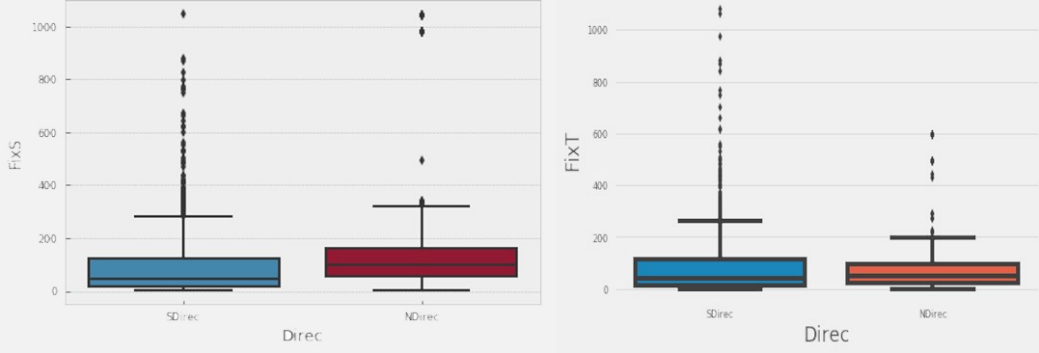
\includegraphics[width=\textwidth]{figures/a2Saedietal-img012.png}
\caption{\label{fig:saedi:10}  The total number of fixations on the source text and target text for same-direction and different-direction language pairs}
\end{figure}

The diminished variation in fixations on the ST for the same-direction language pairs contrasts with the heightened variation for the English-into-Arabic pair, potentially hinting at the complexities introduced by the shift in text orientation during the ST comprehension phase. On the TT front, the patterns intriguingly parallel those observed in the context of script differences. Such elevated variation for the same-direction language pairs might be emblematic of the intricate balance translators strive to achieve between familiarizing themselves with the ST and crafting an accurate rendition in the target language. These findings underscore the profound impact of both script and text direction on the multifarious cognitive processes at play during translation.

The total reading time on the source (TrtS) is shown on the left-side graph in \figref{fig:saedi:11} and the total reading time on the target (TrtT) is shown on the right-side graph of the same figure. For both, the same-direction language pairs (SDirec) show less variation compared to the different-text-direction language pair (SDirec).

\begin{figure}
\label{bkm:Ref148305864}
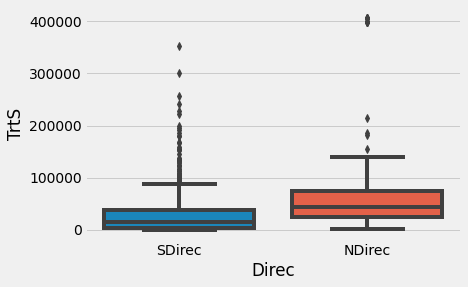
\includegraphics[height=.3\textheight]{figures/a2Saedietal-img013.png}
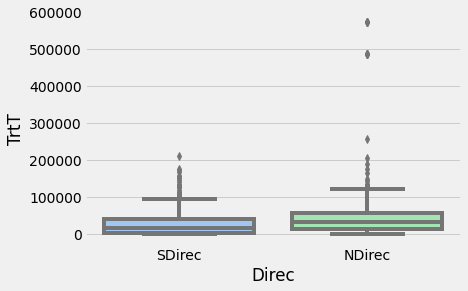
\includegraphics[height=.3\textheight]{figures/a2Saedietal-img014.png}
\caption{\label{fig:saedi:11} Total reading time on the source and target for same-direction and different-direction language pairs}
\end{figure}

The total reading times, as depicted in \figref{fig:saedi:11}, elucidate another dimension of the cognitive processes influenced by text direction during translation. The constricted variation in reading times for the same-direction language pairs contrasts starkly with the broader spectrum exhibited by the English-into-Arabic language pair. Such a distinction indicates a more uniform and possibly streamlined engagement with the ST and TT for translations that maintain consistent text direction. In contrast, the English-into-Arabic pair, with its shift to a right-to-left writing system, presents a more varied engagement, potentially reflective of challenges or pauses for comprehension and production as translators negotiate the shift in text orientation. This variance in reading times, particularly on the ST, might also suggest different translation practices, wherein the same-direction language pairs allow for a steadier translation flow, while the different-direction language pair necessitates longer orientation phase and periodic online revision and final reassessments of the TT based on the ST to ensure translation quality.

\newpage
The last indicator of cognitive effort for text direction is the normalized HTot. \figref{fig:saedi:12} shows more translation variation (HTotN) for the same-text-direction English-into-Spanish and English-into-Chinese language pairs in blue than the different-text-direction English-into-Arabic language pair in red.

\begin{figure}
\label{bkm:Ref148305927}
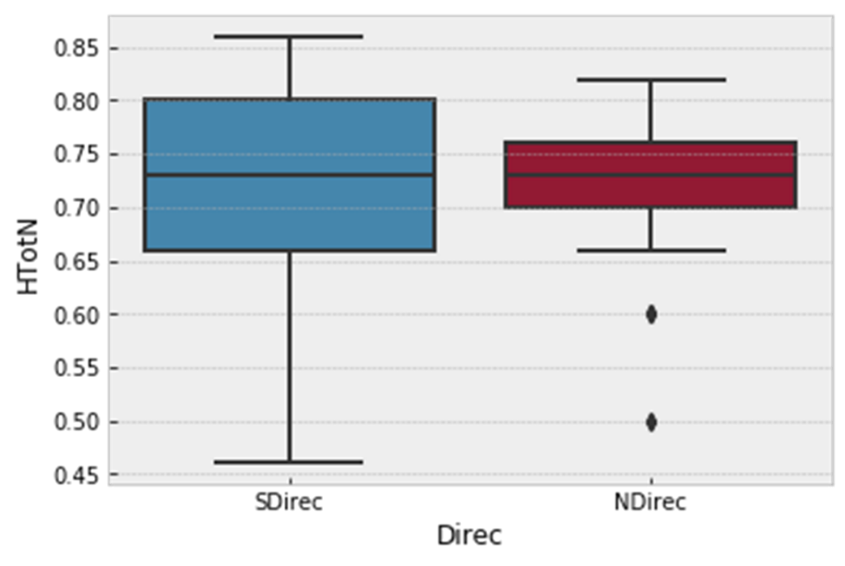
\includegraphics[height=.3\textheight]{figures/a2Saedietal-img015.png}
\caption{\label{fig:saedi:12} Normalized HTot for same-direction and different-direction language pairs}
\end{figure}

The heightened variation observed in the same-direction language pairs (especially English-into-Chinese) could be indicative of a broader spectrum of translational alternatives or strategies employed by translators. This might suggest that when the spatial framework remains consistent across source and target languages, translators might be more inclined to explore a range of interpretative possibilities, leading to a more varied translational output. Conversely, the constricted variation for the English-into-Arabic pair, characterized by its right-to-left text direction, could indicate a more uniform translation approach. Such uniformity might arise from the inherent challenges of reconciling the spatial disparities between ST and TT, compelling translators to adopt a more constrained set of translational strategies to ensure coherence and quality. This dichotomy between the two groups underscores the profound influence of text direction on the cognitive and strategic landscape of translation, suggesting that spatial frameworks significantly modulate translational choices and cognitive engagement.

The discernible variations in cognitive effort across different text directions, as elucidated through multiple indicators, underscore the imperative to adapt translation pedagogy accordingly. Recognizing the heightened cognitive demands when translating into languages with different text directions, curricula should incorporate tailored exercises that specifically target the challenges of different text direction, helping students acclimatize to the spatial adjustments necessitated by such translations. Moreover, given the more constrained translational approach observed for the English-into-Arabic pair, there is a pedagogical opportunity to introduce tools or techniques that aid in navigating the unique challenges of such directionally divergent translations. For instance, intensive training on segmenting the ST into larger chunks during translation might reduce the cognitive load associated with navigating between different text directions. Finally, integrating these insights into classroom discussions can foster an environment of informed awareness, ensuring that future translators are cognitively attuned to the nuanced demands posed by text direction in translation.

\subsection{Interaction effect}

After verifying that both script and text direction have influence on translation effort, we test to see if there is an interaction effect between script and direction affecting effort exerted by translators. This is carried out by conducting a 2-way ANOVA with script and text direction as independent variables and the normalized HTot as the dependent variable. As can be seen in \tabref{tab:saedi:3}, the P values (PR(>F) for both script (Script) and text direction (Direc) are below 0.05. However, the P value for script and text direction interaction (Script:Direc) is above 0.05, which suggests no interaction influence.

\begin{table}
\begin{tabularx}{\textwidth}{Xrrrrr}
\lsptoprule
 & { df} & { sum\_sq} & { mean\_sq} & { F} & { PR(>F)}\\
 \midrule
{ Script} & {{1.0}} & {{3.079041}} & {{3.079041}} & {{455.786561}} & {{5.736319e-85}}\\
{ Direc} & {{1.0}} & {{0.658369}} & {{0.658369}} & {{97.457595}} & {{4.355329e-22}}\\
{ Script:Direc} & {{1.0}} & {{3.5e-05}} & {{3.5e-05}} & {{0.005203}} & {{9.425092e-01}}\\
{ Residual} & {{1107.0}} & {{7.478278}} & {{0.006755}} &  & \\
\lspbottomrule
\end{tabularx}
\caption{\label{tab:saedi:3}The interaction effect of differences in script and text direction in language pairs on cognitive effort}
\end{table}

In addition, the analysis yielded significant main effects for both script and text direction on all other indicators of cognitive effort utilized for purposes of this study, suggesting that these factors independently contribute to increased translation effort. However, there was no significant interaction effect between script and text direction, implying that the cognitive challenges posed by script differences and text direction do not amplify each other when they co-occur (see \tabref{tab:saedi:4} below).

\begin{table}
\begin{tabularx}{\textwidth}{Xrrr}
\lsptoprule
{Indicator} & {Script (p-value)} & {Direc (p-value)} & {Script:Direc (p-value)}\\
\midrule
{PWR} & < 0.00001 & < 0.00001 & 0.950\\
{FixS} & 0.00001 & 0.00004 & 0.389\\
{FixT} & 0.00199 & 0.40293 & 0.75881\\
{TrtS} & < 0.00001 & < 0.00001 & 0.77947\\
{TrtT} & < 0.00001 & 0.0000003 & 0.88705\\
\lspbottomrule
\end{tabularx}
\caption{\label{tab:saedi:4}Two-way ANOVA results for cognitive effort indicators}
\end{table}

The results from the 2-way ANOVAs indicate significant main effects for both script and text direction. This suggests that translating between different-script language pairs (e.g., English into Chinese) and different-direction language pairs (which are also different-script, e.g., English into Arabic) both independently contribute to increased translation effort when compared to translations between similar-script pairs (e.g., English into Spanish). However, the interaction effect between script and text direction is found to be insignificant. This finding is particularly intriguing given that different-text-direction language pair, English into Arabic, inherently involves different scripts as well. One might expect the challenges of script differences to be compounded when paired with different text directions. However, the lack of a significant interaction suggests that the challenges introduced by differing scripts and differing text directions might not amplify each other in a combined scenario. The cognitive processes associated with navigating script differences may be distinct from those required to manage changes in text direction. For instance, while different scripts introduce challenges related to lexical and orthographic shifts, changes in text direction might pose distinct challenges in spatial orientation and processing. The translators might be adept at compartmentalizing these challenges, tackling each in isolation even when both are present, thereby preventing an interaction effect in translation effort.

\subsection{{Final}  {remarks}}

In the realm of translation studies, the intricate interplay between script and text direction, and the ensuing effort, has remained a relatively uncharted territory. Our exploration into this nexus sought to shed light on effort complexities that translators grapple with when confronted with language pairs of different scripts and text direction. Our empirical findings suggest that translating between languages of different scripts, such as English into Chinese or Arabic, indeed imposes heightened cognitive and technical demands, as compared to translations between orthographically similar languages like English into Spanish. This observation aligns with previous assertions, which emphasize the cognitive intricacies tied to orthographic transfer and semantic processing. A different script introduces challenges at orthographic, lexical, and syntactic levels, demanding more intricate cognitive engagement for accurate and fluent translation. Furthermore, the distinction in text direction, as observed in the English-into-Arabic translation scenario, augments demand. Such findings underscore the profound role of spatial orientation in translation. Different text directions compel translators to reconcile not just linguistic but also spatial disparities, thereby magnifying the cognitive load.

However, one of the most intriguing revelations from our study was the absence of a significant interaction between script difference and text direction difference. While both factors individually heightened translation effort, they did not amplify each other’s impact. This suggests that the cognitive processes associated with navigating script differences might be largely distinct from those managing changes in text direction. Such a distinction has profound implications for translation pedagogy. It suggests that training programs should address these challenges separately, offering strategies tailored to each challenge rather than a one-size-fits-all approach. From a pedagogical standpoint, our findings hold considerable ramifications. Given the delineated challenges, translation curricula could benefit from modules focusing on strategies specific to navigating script and text direction differences. This might include exercises tailored to familiarizing students with the nuances of different scripts and spatial orientations and leveraging translation techniques to help manage these challenges.

Our investigation contributes to translation research by providing empirical insights into areas previously underexplored. It elucidates the multifaceted nature of cognitive engagement in translation, emphasizing that beyond linguistic intricacies, spatial and scriptural attributes of languages play a pivotal role. For practice, our findings advocate for a more targeted approach to translator training and professional development. Recognizing the distinct challenges introduced by script and text direction differences, translation agencies might consider offering specialized training or resources to translators handling such language pairs. Another consideration is to account for these challenges in discussions about translator compensation, reflecting the varying complexities introduced by such differences in translation when dealing with such language pairs. Moreover, integrating certain computer-assisted translation (CAT) tools or translation technology could be invaluable in assisting translators in navigating these challenges and improving productivity. For instance, optimal segmentation at a granular level could potentially mitigate the cognitive effort associated with differences in text direction when navigating between ST and TT. Another example is the provision of bilingual term bases for specialized terminologies, which may be particularly beneficial in reducing effort when engaging with language pairs of different scripts and text directions.

Nonetheless, our investigation possesses certain limitations. The specificity of our selected language pairs could circumscribe the broader applicability to a more diverse linguistic spectrum. These delineated constraints underscore pertinent directions for subsequent research endeavors. While the challenges of script and text direction differences are formidable, understanding them paves the way for more informed, effective translation practices and pedagogical approaches. Future research endeavors might delve deeper into the underlying cognitive mechanisms, further enriching our understanding with more factors that might influence translation difficulty. Given the discussion points explored in the present study, detailed, granular qualitatively driven analyses could offer enhanced insights, further corroborating our findings and elucidating the subtleties of effort associated with script and text direction in contrast to other linguistic characteristics inherent to language specificity. Future investigations could also explore whether technical effort is a pivotal factor in measuring translation difficulty.

\section*{Abbreviations}




\begin{tabularx}{.45\textwidth}{lQ}
ST & Source text\\
TT & Target text\\
L1 & First language\\
L2 & Second language\\
Ins & Insertions\\
Del & Deletions\\
Nedits & The overall number of edits\\
DurLog & The logarithm of the production duration\\
PWR & Pause-to-word ratio\\
\end{tabularx}
\begin{tabularx}{.49\textwidth}{lQ}
FixS & The total number of fixations on the source text\\
FixT & The total number of fixations on the target text\\
TrtS & Tthe total reading time on the source text\\
TrtT & The total reading time on the target text\\
HTot & The total translation entropy\\
\\
\end{tabularx}
\sloppy\printbibliography[heading=subbibliography,notkeyword=this]
\end{document}
